%!TEX program = xelatex
%%%%%%%%%%%%%%%%%%%%%%%这是导言部分的开始%%%%%%%%

%========= 导言部分声明文档的类型=================
\documentclass{article}

	%=========导言部分可可以加载宏包=================
	\usepackage{amsmath}                % 数学公式排版宏包
	\usepackage{amssymb}                % 数学符号命令宏包
	\usepackage{amsthm}                 % 数学定理宏包
	\usepackage[UTF8]{ctex}             % 中文输入宏包
	\usepackage[a4paper]{geometry}      % 页面设置宏包
	\usepackage{setspace}               % 行间距宏包
	\usepackage{graphicx}               % 图片宏包
	\usepackage{listings}               % 代码宏包
	\usepackage{color}					% 颜色宏包
	\usepackage{xcolor}                 % 颜色处理宏包
	\usepackage{float}                  % 浮动对象式样宏包
	\usepackage{fontspec}
	\usepackage{enumerate}				% 列举编号包
	
	%=========页面设置==============================
	\geometry{left=1cm,right=1cm,top=1cm,bottom=2cm}
	\onehalfspacing
	\setlength\parindent{0em}

	%=========代码格式设置============================
	\definecolor{dkgreen}{rgb}{0,0.6,0}
	\definecolor{gray}{rgb}{0.5,0.5,0.5}
	\definecolor{mauve}{rgb}{0.58,0,0.82}
	% \setmonofont{Consolas}
	\lstset{
		numbers = left, 	
		numberstyle = \color{gray}, 
		keywordstyle = \color{blue},
		commentstyle = \color{dkgreen}, 
		stringstyle = \color{mauve},
		basicstyle = \ttfamily,
		breaklines = true,
		frame = shadowbox, % 阴影效果
		rulesepcolor = \color{ red!20!green!20!blue!20} ,
		escapeinside = ``, % 英文分号中可写入中文
		xleftmargin = 2em,xrightmargin=2em, aboveskip=1em,
		framexleftmargin = 2em
	} 

%=========导言部分可以定义标题信息===============
\title{组会报告}
\author{徐益}
\date{\today}
%%%%%%%%%%%%%%%%%%%%%%%这是导言部分的结束%%%%%%%%%

%%%%%%%%%%%%%%%%%%%%%%%这是正文部分的开始%%%%%%%%%
\begin{document}

%=========生成标题================================
\maketitle

%=========开始正文的输入==========================

%===========第一节=================
\section{工作内容}
1. 实现基于C的avx2-OMS译码测试平台;

2. 提高avx2-OMS吞吐量。

%===========第一节=================
\section{提高avx2-OMS吞吐量的具体方法}
\subsection{改变数据结构使内存空间连续}
原数据结构:
\lstset{language=C++}
\begin{lstlisting}
typedef struct check_node
{
	int8_t degree;		// number of connective variable nodes
	int16_t *index;		// index of connective variable nodes
	float* message;		// message from cn to vn
	int8_t* message_fixed;	// fixed message from cn to vn
	__m256i* message_avx2;	// avx2 message from cn to vn
	int8_t pointer;		// pointer to the message that will be used
} check_node;
\end{lstlisting}
现数据结构:
\lstset{language=C++}
\begin{lstlisting}
typedef struct nr15_ldpc_simd_t
{
	......
	int8_t* degree;	// number of connective check nodes(length:M)
	int16_t* index;	// index of connective check nodes(length:M_whole)
	__m256i* cn_msg_avx2;	// avx2 message from cn to vn(length:M_whole)
	__m256i* llr_avx2;	// avx2 llr(length:N)
	__m256i** llr_addr;	// llr address from cn to vn(length:M_whole)
	__m256i* vn_msg_avx2;	// temp avx2 message from vn to cn(length:19)
} nr15_ldpc_simd_t;
\end{lstlisting}

\subsection{使用更小的校验矩阵}
\begin{figure}[H]
	\centering
	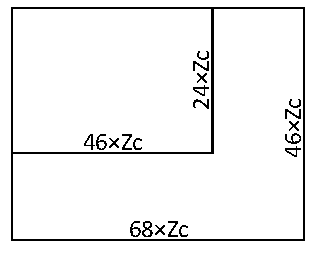
\includegraphics[width = .4\textwidth]{H.pdf}
	\caption{优化前后校验矩阵尺寸变化}
\end{figure}

\subsection{编译方式的优化}
\begin{figure}[H]
	\centering
	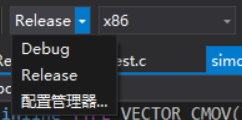
\includegraphics[width = .4\textwidth]{release.png}
	\caption{项目版本的选择}
\end{figure}
\begin{figure}[H]
	\centering
	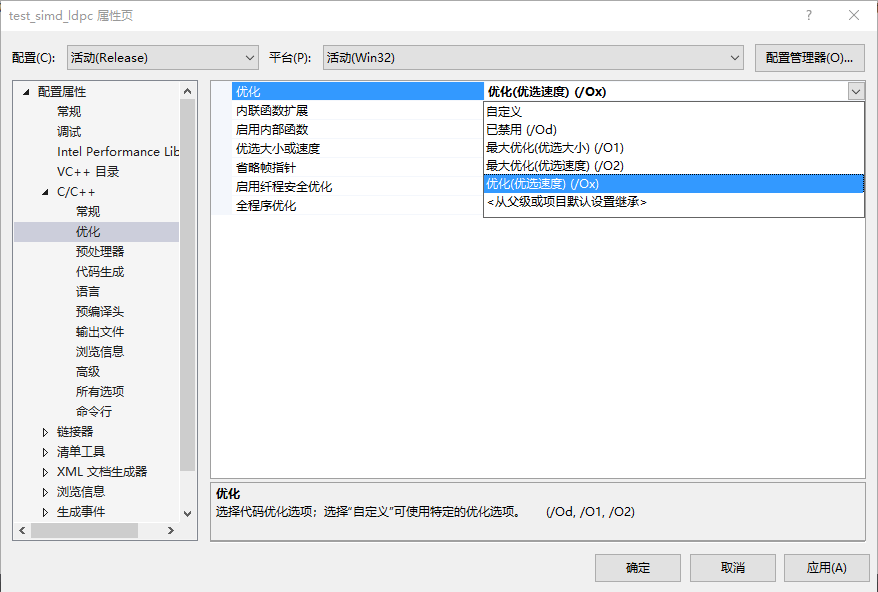
\includegraphics[width = .8\textwidth]{ox.png}
	\caption{优化方式的选择}
\end{figure}

\subsection{限幅部分的优化}
\lstset{language=C++}
\begin{lstlisting}
for (r = 0; r < C; r++)
	for (n = 0; n < Nd / 8; n++)
	{
		resf = _mm256_mul_ps(*p_tabI, fact);
		resf = _mm256_max_ps(resf, vminf);
		resf = _mm256_min_ps(resf, vmaxf);
		resi = _mm256_cvttps_epi32(resf);
		p_tabI += 1;
		for (i = 0; i < 8; i++)
			ptr_llr[32 * (8 * n + i) + r] = (int8_t)p_resi[i];
	}
\end{lstlisting}

\subsection{判决部分的优化}
\begin{lstlisting}
uchar_itranspose_avx(h->llr_avx2, (__m256i*)decoded_bits, K);
\end{lstlisting}

%===========第二节=================
\section{VTune测试结果分析}
\subsection{吞吐量计算}
\begin{figure}[H]
	\centering
	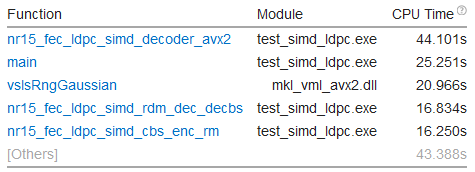
\includegraphics[width = .8\textwidth]{res.png}
	\caption{Top Hotspots in VTune}
\end{figure}
$B=(8448-24)*32*10^5=2.6957Gbit$\\
$t=44.101s$\\
$Throughput=B/t=2.6957Gbit/44.101s=61.125Mbps$

\subsection{主要耗时部分}
\subsubsection{循环1}
\begin{figure}[H]
	\centering
	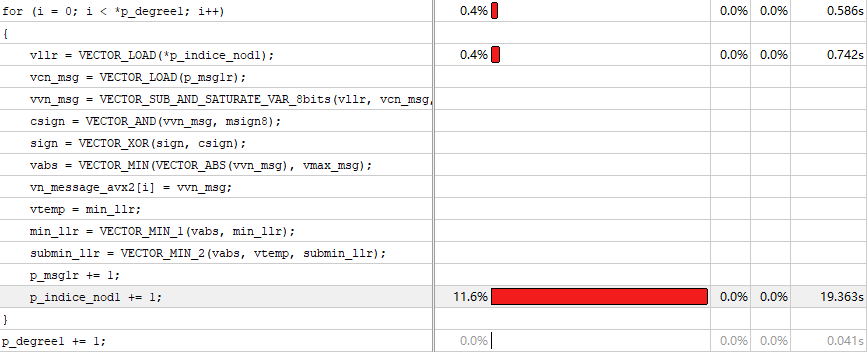
\includegraphics[width = .8\textwidth]{loop1.png}
	\caption{循环1耗时情况}
\end{figure}
\subsubsection{循环2}
\begin{figure}[H]
	\centering
	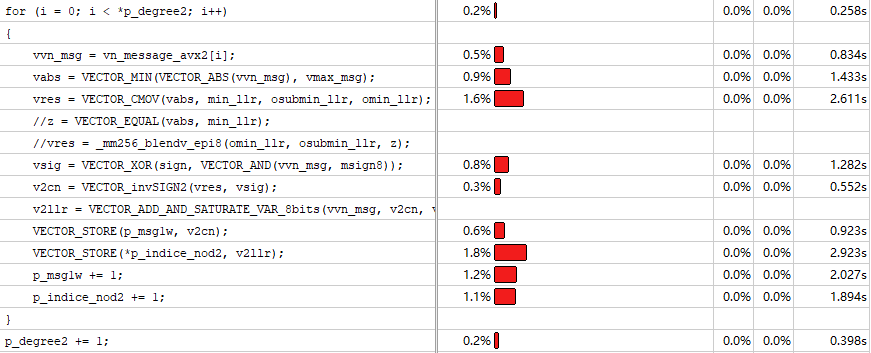
\includegraphics[width = .8\textwidth]{loop2.png}
	\caption{循环2耗时情况}
\end{figure}
\subsubsection{限幅部分}
\begin{figure}[H]
	\centering
	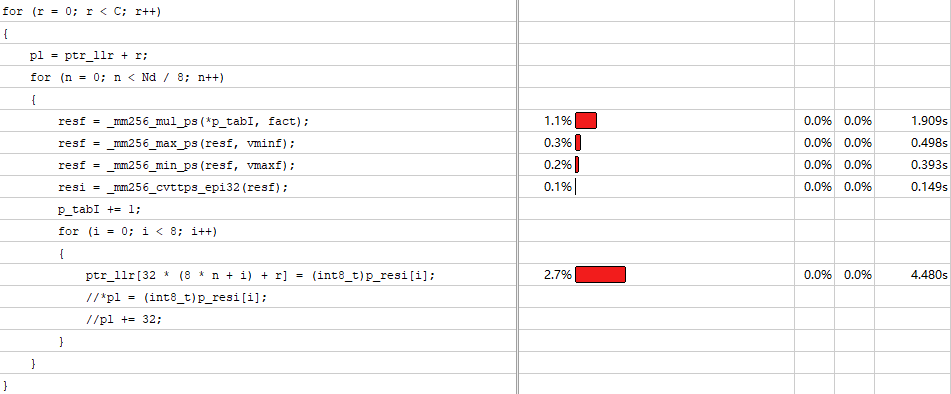
\includegraphics[width = .8\textwidth]{fix.png}
	\caption{限幅部分耗时情况}
\end{figure}

%===========第三节=================
% \section{尝试解决fixed-OMS译码曲线出现的“平台”现象}
% \subsection{消除float转int8\_t时inf造成的影响}


%===========第四节=================
% \section{仍存在问题}


%===========下周计划=================
% \section{下阶段计划}
% 1. 进一步优化吞吐量性能

\end{document}
%%%%%%%%%%%%%%%%%%%%%%%这是正文部分的结束%%%%%%%%%%%%